\subsection{Prétraitements Statistiques}

Avant d'alimenter l'algorithme de fusion de données, il est indispensable de traiter les signaux bruts afin d'éliminer les biais matériels et les valeurs aberrantes majeures

\subsubsection{Nettoyage des données GPS}
\begin{itemize}
    \item[$\bullet$] \textbf{Temps de chauffe (Warm-up)} : Les 15 premières secondes d'acquisition GPS sont systématiquement ignorées. Ce délai permet au récepteur GNSS d'acquérir un nombre suffisant de satellites pour converger vers une solution de positionnement stable.
    \item[$\bullet$] \textbf{Filtrage statistique IQR} : Nous appliquons la méthode de l'Écart Interquartile (IQR) sur les colonnes de latitude et de longitude. Les coordonnées tombant en dehors de l'intervalle $[Q_1 - 1.5 \times IQR, Q_3 + 1.5 \times IQR]$ sont identifiées comme des erreurs de mesure extrêmes (outliers) et sont éliminées.
\end{itemize}



\subsection{Modèle Cinématique du Filtre de Kalman Étendu (EKF)}
\label{sec:ekf}

Après de multiples essais, nous avons abandonné la double intégration de l'accélération (trop de dérive due à la gravité et des erreurs priovenant de l'imu) et l'usage du magnétomètre (trop d'interférences magnétiques extérieures qui fausse les estimations de ekf). Notre modèle cinématique s'appuie désormais uniquement sur la vitesse scalaire calculée a partir des données du GPS ($v$) et la vitesse de rotation autour de l'axe vertical donnée par le gyroscope ($\omega$).

\subsubsection{Vecteur d'État et Commande}
Nous modélisons le piéton dans un plan 2D local (repère Est-Nord). Le vecteur d'état $X_k$ à l'instant $k$ contient 3 variables :
\begin{equation}
 X_k = \begin{bmatrix} x_k \\ y_k \\ \theta_k \end{bmatrix} 
\end{equation}
Où $x_k$ et $y_k$ sont les positions vers l'Est et le Nord (en mètres), et $\theta_k$ est le cap (en radians, où 0 = pointé vers l'Est).

\begin{figure}[htbp]
    \centering
    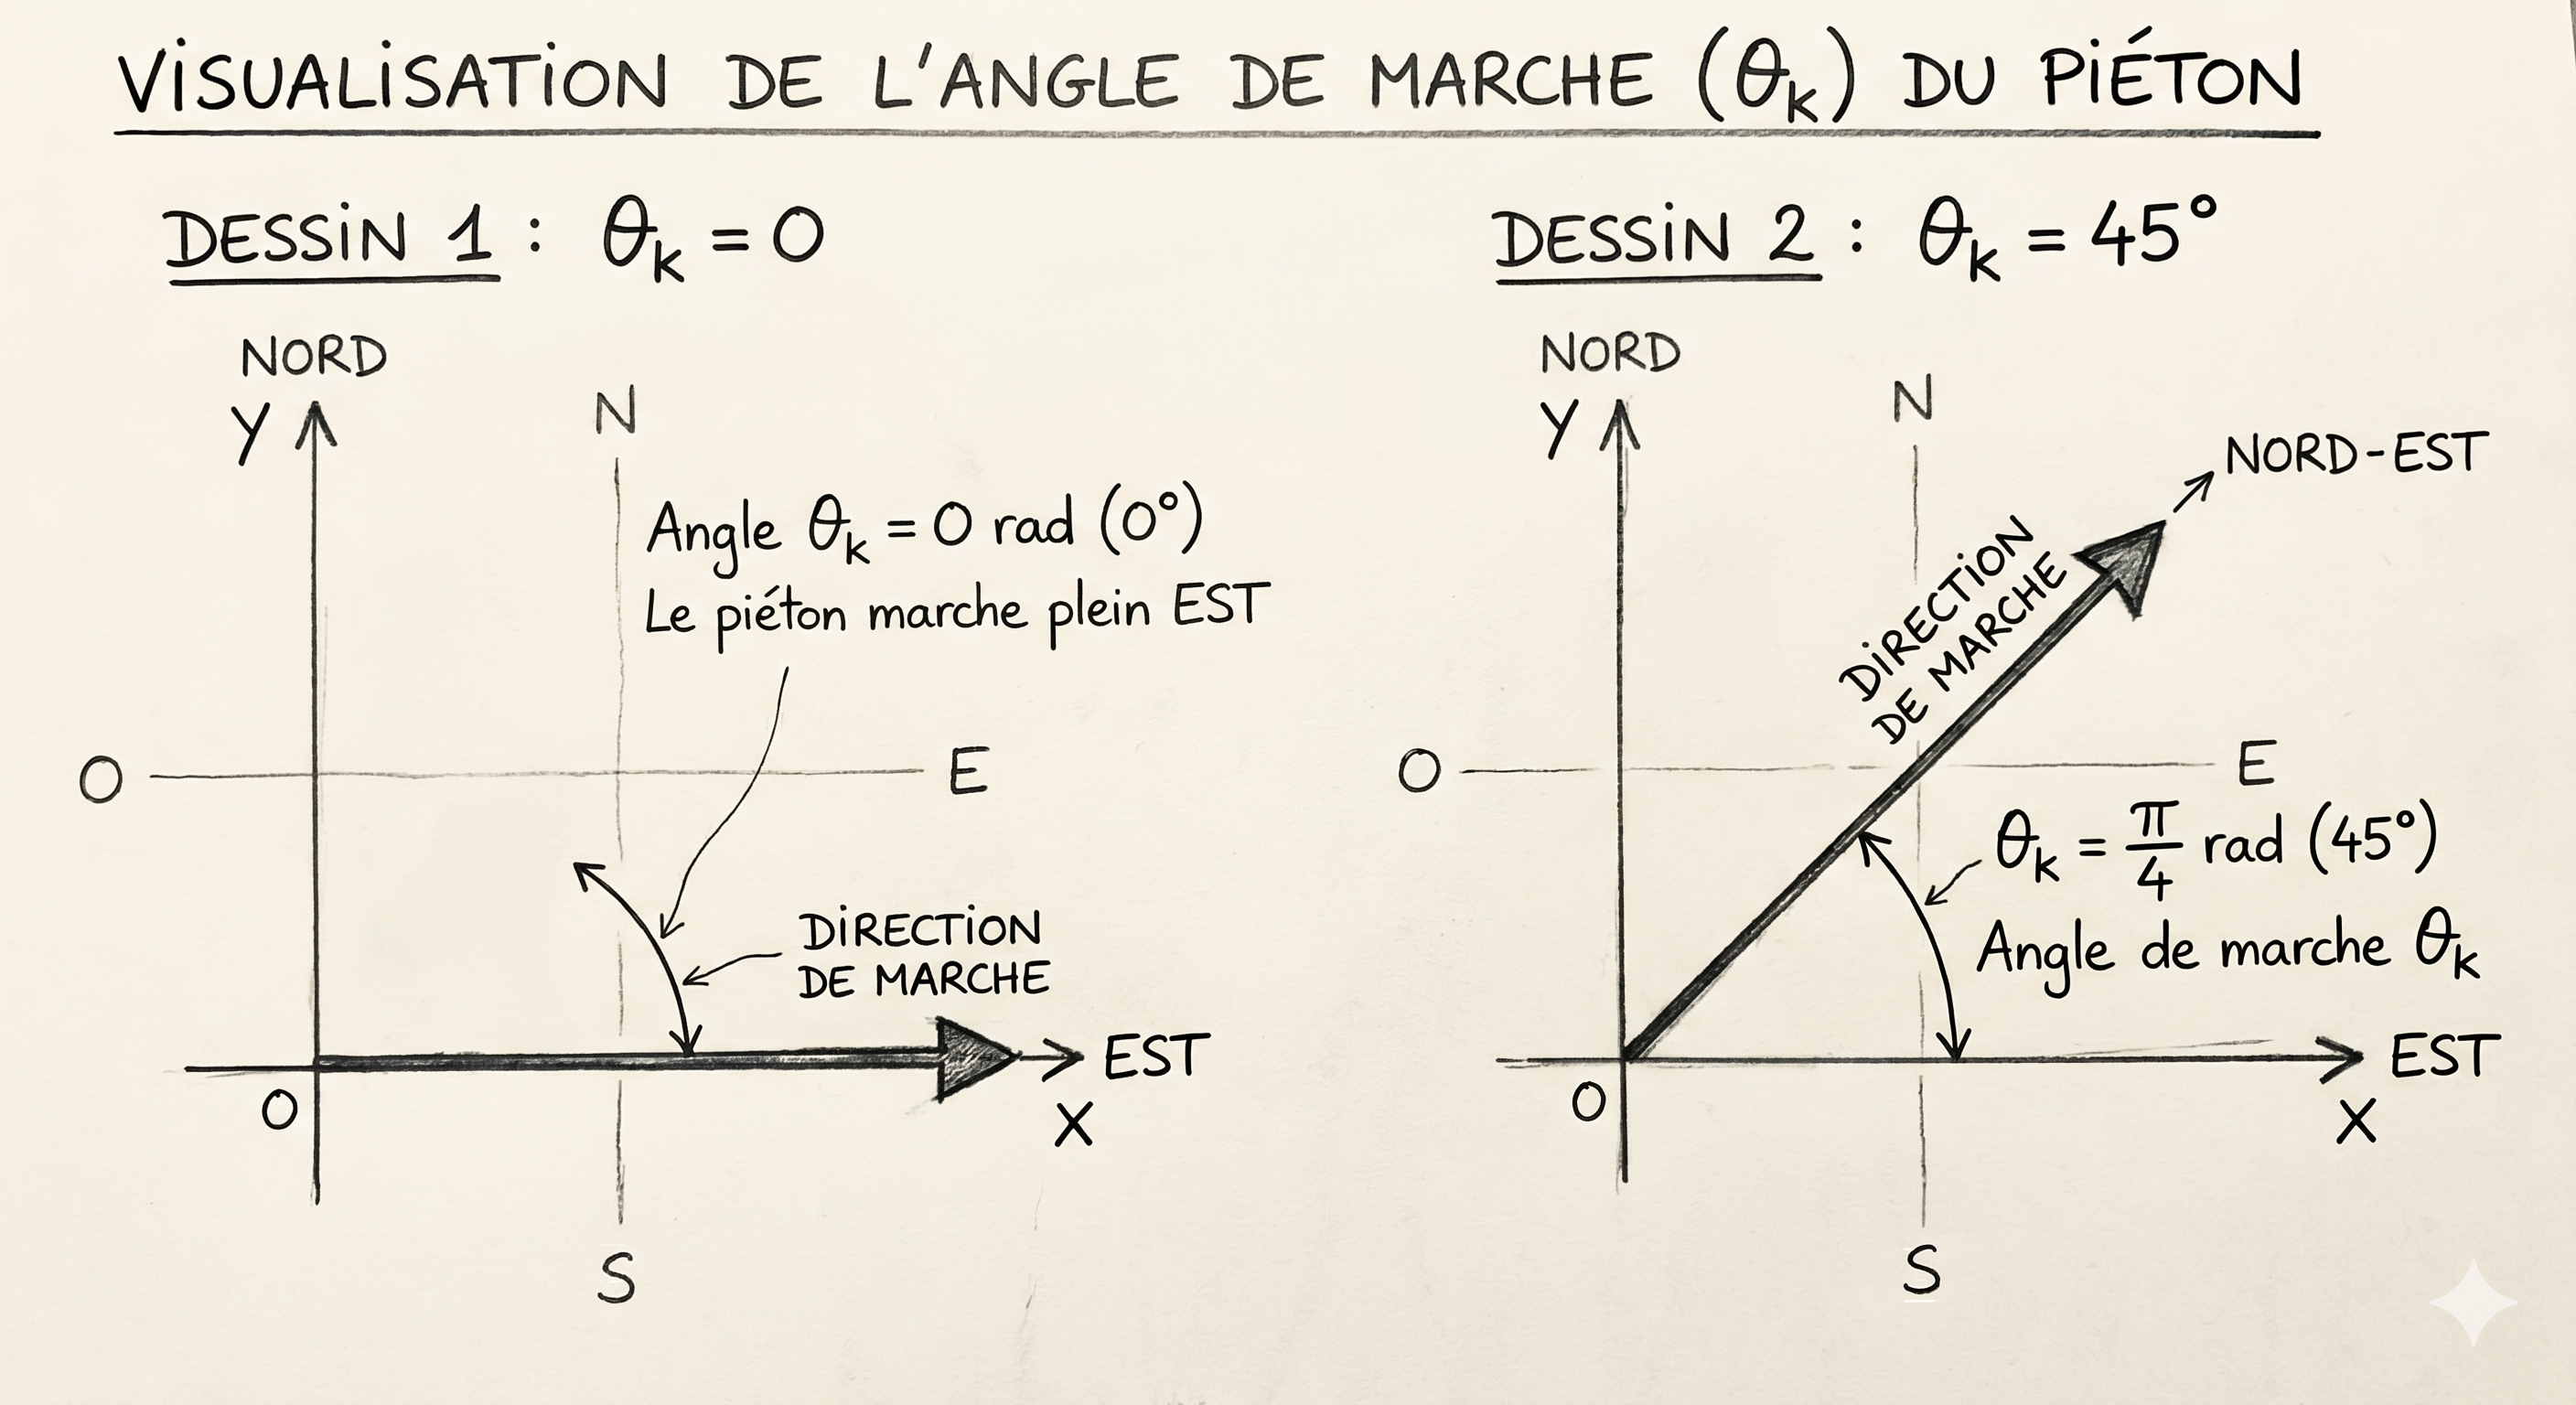
\includegraphics[width=0.5\textwidth]{images/model_boussole.png}
    \caption{Modèle de la boussole et repère Est-Nord}
    \label{fig:model_boussole}
\end{figure}

Le système est piloté par le vecteur de commande $U_k$ :
\begin{equation}
 U_k = \begin{bmatrix} v_k \\ \omega_k \end{bmatrix} 
\end{equation}
Où $v_k$ est la vitesse scalaire du piéton et $\omega_k$ la vitesse angulaire. 
Dans notre montage matériel, nous avons observé expérimentalement que l'accéléromètre mesurait systématiquement environ $1G$ (la gravité terrestre) sur l'axe X, tandis que les axes Y et Z restaient proches de $0G$. On en deduit que la carte Raspberry Pi était fixée de sorte que son axe X pointait verticalement vers le ciel. Donc la rotation du piéton sur lui-même correspond physiquement à une rotation autour de cet axe vertical, qui est lue directement par \textit{Gyro\_X} (IMU).

\begin{figure}[htbp]
    \centering
    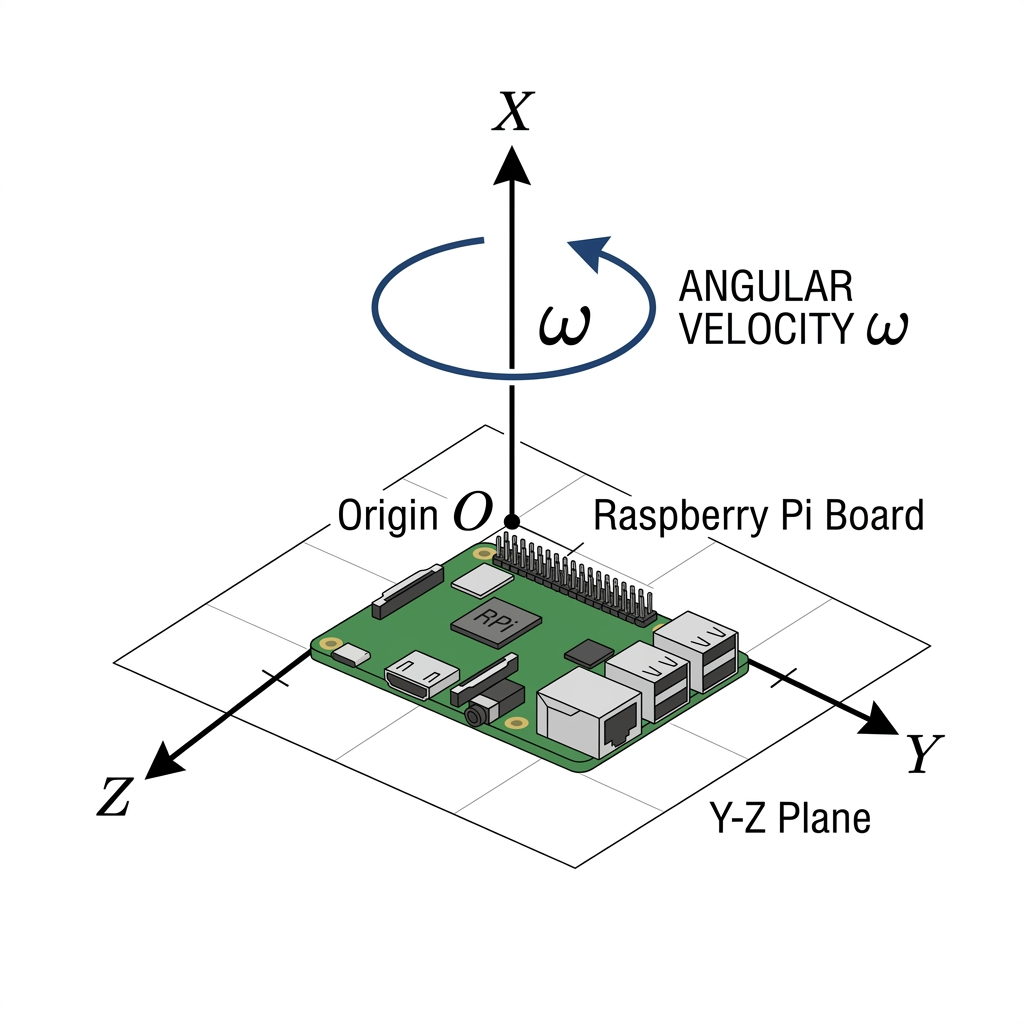
\includegraphics[width=0.5\textwidth]{images/diagramme_imu_axe_x.png}
    \caption{Montage matériel de l'IMU : l'axe X pointe vers le haut}
    \label{fig:diagramme_imu_axe_x}
\end{figure}

\subsubsection{Étape de Prédiction (Propagation)}
L'évolution de la position du piéton n'est pas linéaire à cause des fonctions trigonométriques. Le modèle non-linéaire $f$ se traduit par les équations de mécanique classique :
\begin{equation}
 \begin{bmatrix} x_k \\ y_k \\ \theta_k \end{bmatrix} = \begin{bmatrix} x_{k-1} + v_k \cdot \cos(\theta_{k-1}) \cdot \Delta t \\ y_{k-1} + v_k \cdot \sin(\theta_{k-1}) \cdot \Delta t \\ \theta_{k-1} + \omega_k \cdot \Delta t \end{bmatrix} 
\end{equation}

\begin{figure}[htbp]
    \centering
    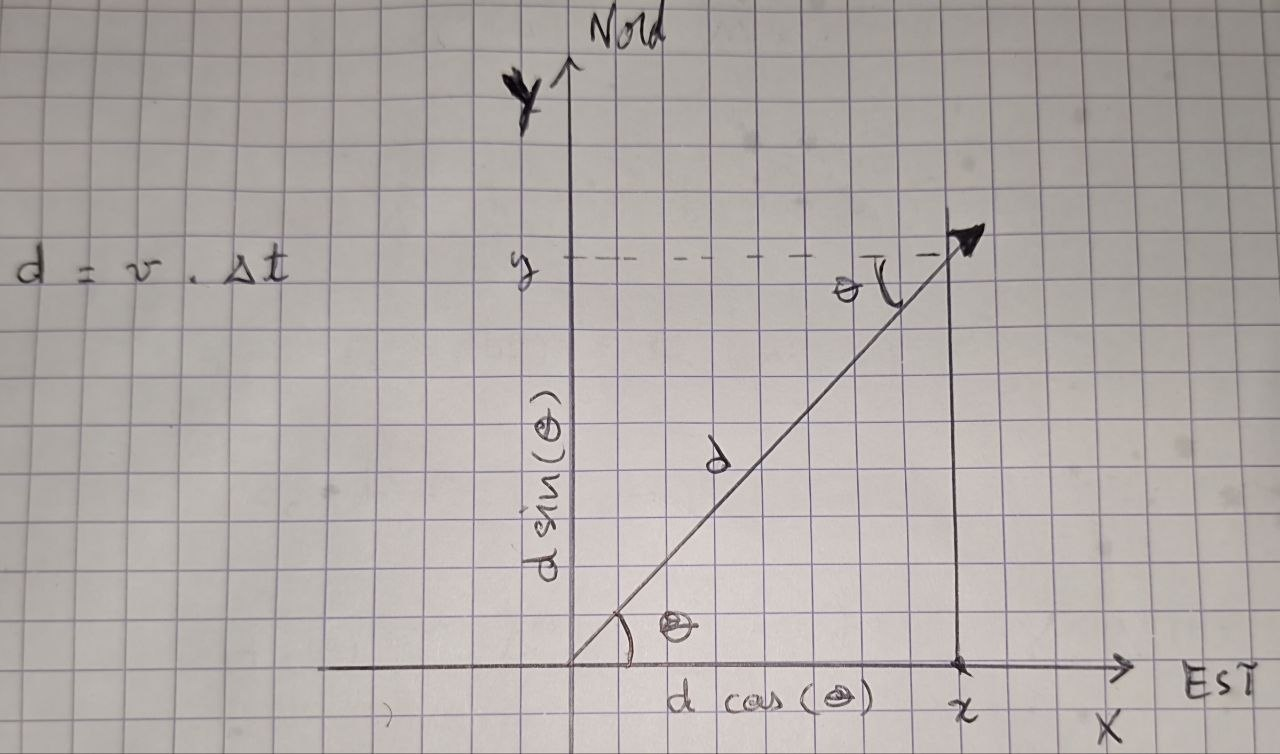
\includegraphics[width=0.5\textwidth]{images/trigo_cinematique.jpg}
    \caption{Projection trigonométrique du déplacement $v \cdot \Delta t$ sur les axes Est ($X$) et Nord ($Y$)}
    \label{fig:trigo_cinematique}
\end{figure}

Pour appliquer le filtre de Kalman, nous devons linéariser cette fonction en calculant sa Jacobienne $F_k$ :
\begin{equation}
 F_k = \frac{\partial f}{\partial X} = \begin{bmatrix} 1 & 0 & -v_k \cdot \sin(\theta_{k-1}) \cdot \Delta t \\ 0 & 1 & v_k \cdot \cos(\theta_{k-1}) \cdot \Delta t \\ 0 & 0 & 1 \end{bmatrix} 
\end{equation}

\textbf{Matrice de Bruit de Processus ($Q$)} \\
La matrice de covariance $Q$ représente l'incertitude de notre prédiction. Issue du modèle \textbf{CWNA} (\textit{Continuous White Noise Acceleration}, réf. CM6), elle se modélise par :
\begin{equation}
 Q = \begin{bmatrix} \frac{\sigma_a^2 \cdot \Delta t^4}{4} & 0 & 0 \\ 0 & \frac{\sigma_a^2 \cdot \Delta t^4}{4} & 0 \\ 0 & 0 & \sigma_\omega^2 \cdot \Delta t^2 \end{bmatrix} 
\end{equation}
Ici, $\sigma_a$ est recalculé dynamiquement à chaque itération via la variance de l'accélération horizontale de l'IMU, permettant au filtre de s'adapter à la force réelle du pas de l'utilisateur.
La prédiction de la covariance devient alors : $P_{k|k-1} = F_k P_{k-1|k-1} F_k^T + Q$.

\subsubsection{Étape de Correction (Mise à jour GPS)}
Nous mesurons uniquement la position $(x, y)$ grâce au GPS. La matrice d'observation $H$ est donc linéaire :
\begin{equation}
 H = \begin{bmatrix} 1 & 0 & 0 \\ 0 & 1 & 0 \end{bmatrix} 
\end{equation}

La matrice $R$ représente l'imprécision du GPS, obtenue expérimentalement lors de nos tests :
\begin{equation}
 R = \begin{bmatrix} 1.20 & 0 \\ 0 & 0.07 \end{bmatrix} 
\end{equation}

\textbf{Filtre Anti-Outliers (Distance de Mahalanobis)} \\
Afin de rejeter les mesures GPS aberrantes (phénomène de \textit{multipath} ou pertes de signal temporaires), nous avons implémenté une technique de \textit{gating} probabiliste basée sur la distance de Mahalanobis. Avant d'accepter une mesure GPS, nous calculons l'innovation $\tilde{y} = Z_k - H \hat{X}_{k|k-1}$ et sa covariance $S = H P_{k|k-1} H^T + R$.
Nous évaluons ensuite la distance de Mahalanobis au carré : $d^2 = \tilde{y}^T S^{-1} \tilde{y}$. 

Statistiquement, les résidus normalisés d'un filtre de Kalman optimal suivent une loi du $\chi^2$ (Khi-deux). Pour notre système d'observation 2D (X et Y), nous avons 2 degrés de liberté.
Pour rejeter les données aberrantes avec un intervalle de confiance de 99\%, le seuil théorique tabulé est de $9.21$ (\textit{Réf : Tables statistiques du $\chi^2$ / Théorie de l'estimation et du filtrage optimal}). 
Ainsi, si $d^2 > 9.21$, la mesure GPS est considérée comme une anomalie et est purement ignorée, laissant le modèle inertiel prendre le relais pour garantir la fluidité de la trajectoire.

Si la mesure est valide, nous calculons le gain de Kalman $K$ et corrigeons l'état :
\begin{align}
   K &= P_{k|k-1} H^T S^{-1} \\
   \hat{X}_{k|k} &= \hat{X}_{k|k-1} + K \tilde{y} \\
   P_{k|k} &= (I - K H) P_{k|k-1}
\end{align}

\subsection{Critique et Limites du Modèle}

Bien que robuste face aux interférences magnétiques et au bruit d'accélération, notre modèle EKF cinématique repose sur plusieurs hypothèses:

\begin{enumerate}
    \item \textbf{Dépendance à la vitesse déduite du GPS} : Actuellement, la vitesse scalaire $v_k$ est calculée à partir de la différence de position entre deux points GPS successifs. Une amélioration  consisterait à récupérer et utiliser directement la vitesse \textit{Doppler} native fournie par la puce GPS (via les trames NMEA originelles). Cette vitesse matérielle est nettement plus instantanée et fiable que la dérivation spatiale. De plus, si le signal GPS est totalement perdu (ex: tunnel prolongé), notre vitesse calculée tombe à zéro, empêchant toute vraie navigation (mais cela peut se resoudre en integrant temporairement l'acceleration).
    \item \textbf{Dérive résiduelle du Gyroscope (Drift)} : En l'absence d'un cap absolu (le magnétomètre ayant été écarté du modèle en raison des perturbations environnementales), l'intégration numérique de la vitesse angulaire $\omega_k$ finira inévitablement par dériver au bout de plusieurs dizaines de minutes de marche, malgré notre calibration statique du biais initial.
    \item \textbf{Hypothèse de mouvement rectiligne aligné} : Le modèle cinématique suppose que le piéton avance en permanence de manière parfaitement alignée avec l'axe de visée de la carte (cap $\theta$). Cette restriction rend le modèle incapable d'estimer correctement la trajectoire lors de mouvements tels que les pas chassés ou les marches en reculant ... (personne ne fait ça normalement)
\end{enumerate}

Nous avons pas pu exploiter le magnetomètre comme il se devait il resoudrait bon nombre de nos problèmes.